\usechapterimagetrue
\chapterimage{nasa.jpg} % Chapter heading image
\chapter{Data transmission}
\usechapterimagefalse

In the previous chapter we investigated the data compression problem. That is, given a source and some noiseless means of communication, the problem is to encode the source in such a way that we minimize the usage of the noiseless communications channel while we allow the receiver to recover the message. Here we will investigate a dual problem, the problem of transmitting a source over a noisy channel. This problem, is the problem that your mobile phone faces each time that it wants to exchange information with the nearest base station. %, or the problem that your ADSL router faces to transmit information over fiber. 
It is also the same problem that your computer faces when it wants to store information on a disk in such a way that it can be recovered at a later time. %This is as we see a very relevant problem. We will not have the time to dig into great depth, but the menu should allow you to get a solid understanding of the mathematical foundations and a glimpse about how we tackle it currently. In the figure above, you can see the XXXX space XXX. As you can imagine, the bandwidth of the communications channel linking it with earth is very limited, the information we want to exchange precious and the channel rather noisy. Space exploration has been one unexpected driver of progress for pushing the limits of error correcting codes. (why error correting?)
\booksection{The communications problem}
\label{sec:comprob}
\begin{figure}[h!]
\begin{center}
\def\svgwidth{\columnwidth} 
\input{figures/shannoncom.pdf_tex}
\end{center}
\caption[Communications system diagram.]{This figure reproduces the communications system diagram introduced by Shannon~\cite{Shannon_48}.}
\label{fig:shannoncom}
\end{figure}
Let us first of all, depict the building blocks of an idealized communications problem. Our description parallels the one of Shannon~\cite{Shannon_48}, see in Fig.~\ref{fig:shannoncom} a graphical representation. The figure shows five entities: an information source, a transmitter, a noise source, a receiver, and a destination. The communications scheme works as follows: 

First the information source generates a message $m$ from a set of possible messages $M$. Then, the transmitter takes $m$ and encodes it into $n$ channel symbols. We define the coding rate $R$ as:

\begin{equation}
R=\frac{\log M}{n}
\end{equation}

%\begin{exercise}
%Suppose that we want to transmit a message from a set of $16$ messages that a source will choose uniformly at random. We have two channels available, both are noiseless, one allows to transmit one bit per channel use and we can use it once per second. The second channel allows to transmit two bits per channel use and we can use it once per minute. Over which channel can we communicate at a higher rate? How does time influence this number?
%\end{exercise}
The channel is a physical medium of transmission. Mathematically, we can model it as a system taking symbols from input alphabet $\mathcal{X}$ to symbols of output alphabet $\mathcal{Y}$ and characterized by a transition probability matrix that maps the probability of every symbol $y$ if symbol $x$ is sent. The receiver tries to undo the encoding given the noisy received signal and at the end of the scheme the destination receives the ${\hat{m}}$ possibly identical to $m$.

\booksection{Detection, correction and minimum distance}
Let us recall our original example of transmitting the weather forecast. Let us recall that the set of messages is binary : rain and sun. If we are interested in transmitting one of these messages through a noiseless channel, it should be clear that unless one of the two messages has zero probability the encoding with minimum average length will assign to rain the codeword $0$ and to sun $1$ or viceversa. 

Let us now imagine that we want to transmit the weather forecast through a noisy channel. For instance a channel that takes a binary symbol as input and outputs the same symbol with probability $1-p$ or flips it with probability $p$. In this new scenario, unless we change the encoding, the messages transmitted will be erroneous with probability $p$. The most obvious way of protecting against error is repeating the message. 

The repetition code of length $2$ is $C=\{00,11\}$. Now, if one of the bits is flipped, we will receive a word that is not a codeword. With this scheme, we can detect any one bit error. Unfortunately, if we receive the word $01$ it could be that the first bit flipped or that the second bit flipped. In the first case the codeword sent would be $11$, while in the second case $00$. That is, this scheme allows us to detect any one bit error pattern, but not to correct it.

The repetition code of length $3$ is $C=\{000,111\}$. Now, by the same argument as before, we can detect any two bit error pattern. Moreover, if we were guaranteed that at most one error occurred, we could also correct it. For instance, if we receive the word $100$ and we know that at most one error occurred, we can coclude that the codeword $000$ was transmitted.

Now let us imagine that bits are not flipped, but erased with a certain probability, and that when bits are erased they are replaced by an erasure symbol $e$. For instance, if we send the codeword $00$ over a channel that erases each symbol with probability $e$, we could receive the word $0e$ (question: with what probability would we receive it?). The only codeword compatible with $0e$ is $00$ and we can see by inspection that the length two repetition code can correct any error pattern consisting of a single erasure.

In the following we will introduce the necessary definitions to understand quantitatively these previous examples. 

First, we introduce a distance function between vectors.
\begin{definition}
The Hamming distance between two vectors $x,y\in D^n$ is given by:
\begin{equation}
d(x,y)=|{i:x_i\neq y_i, 1\leq i\leq n}|
\end{equation}
\end{definition}
An useful way of interpreting the Hamming distance is as the minimum number of positions that it is necessary to change in $x$ to transform it to $y$.
\begin{example}
The Hamming distance between vectors $x=(1,2,0,1,2)$ and $y=(2,1,0,1,2)$ is two because they differ in the first two entries. Alternatively, from the definition
\begin{equation}
d(x,y)=|{i:x_i\neq y_i, 1\leq i\leq n}|=|{1,2}|=2
\end{equation}\end{example}
A function $d:\mathcal X\times \mathcal X\mapsto \mathbb R$ is a distance function if it verifies the following properties:
\begin{enumerate}
%\item Non-negativity: $d(x,y)\geq 0$
\item Identity: $d(x,y)=0$ if and only if $x=y$
\item Symmetry: $d(y,x)=d(x,y)$
\item Triangle inequality: $d(x,y)\leq d(x,z)+d(z,y)$
\end{enumerate}
\begin{exercise}
Show that the Hamming distance is a valid distance function
\end{exercise}
In the following whenever we refer to a distance, we will refer to the Hamming distance unless explicitly stated otherwise.

The decoding strategy that we described above is called nearest neighbor decoding or minimum distance decoding. A minimum distance decoder is a decoder that outputs the codeword closest in distance to the received vector $y$, or in the case that there are more than one it will choose from the set of closest codewords uniformly at random.
\begin{equation}
\text{dec}(x) = \argmin_{x\in C}d(x,y)
\end{equation}
\begin{example}
A minimum distance decoder for the repetition code of length 3 will output 000 when it receives as input the word $001$ since $000$ has a smaller hamming distance to $001$ than the other codeword in the code: $111$.
\end{example}

Now we introduce block codes. In the previous chapter we mostly worked with variable length codes. For error correction, we will restrict our analysis to codes with all codewords of the same length.
\begin{definition}
A binary block code is a function $C:\{0,1\}^k\mapsto \{0,1\}^n$, where $k\geq n$ are natural numbers.
\end{definition}

%\booksection{The repetition code and two simple channels}
To understand the behavior of a decoder quantitatively we need to introduce measures of failure and success. The error probability of a codeword $x$ is the probability that a decoder outputs a codeword different than $x$. 
\begin{equation}
p_e(x)=\sum_{y\in \{0,1\}^n}p(y|x)p(\text{dec}(y)\neq x)
\end{equation}
and the error rate of a code:
\begin{equation}
p_e(C)=\sum_{w\in C}p(w)p_e(w)
\end{equation}

Let us now study the effect of the repetition code in error rate on two important communications channels.

\begin{exercise}
\label{ex:bsc}
Consider $C=\{000,111\}$, suppose that we send each symbol of the word 000 through a BSC$(p)$.
\begin{itemize}
\item What is the probability of having no errors?
\item What is the probability of having one error?
\item What is the probability of having two errors?
\item What is the probability of having three errors?
\item What is the error probability with a minimum distance decoder?
\end{itemize}
\end{exercise}

\begin{exercise}
\label{ex:bec}
Consider $C=\{000,111\}$, suppose that we send each symbol of the word 000 through a BEC$(p)$.
\begin{itemize}
\item What is the probability of having no erasures?
\item What is the probability of having one erasure?
\item What is the probability of having two erasures?
\item What is the probability of having three erasures?
\item What is the error probability with a minimum distance decoder?
\end{itemize}
\end{exercise}

From solving the previous two exercises you can realize that the performance of the minimum distance decoder is linked to the minimum distance between all codewords. This is an important metric for a code and we will use the following notation:

\begin{equation}
d_{\min}(C)=\min_{x,y\in C,x\neq y}d(x,y)
\end{equation}

Now, let us make explicit this intuition with the following set set of exercises. Recall that the number of strings of length $n$ with $k$ ones is $n\choose k$.
\begin{exercise}
Show that a code $C$ can detect all error patterns with $s$ errors if and only if $d_{\min}(C)\geq s+1$
\end{exercise}
\begin{exercise}
Show that a code $C$ can correct all error patterns with $t$ errors if and only if $d_{\min}(C)\geq 2t+1$
\end{exercise}

\begin{exercise}
Show that a code $C$ can detect all erasure patterns with $e$ errors if and only if $d_{\min}(C)\geq e+1$
\end{exercise}

\begin{exercise}
Given a code with minimum distance 12, find the maximum number of errors it can detect, the maximum number of errors it can correct and the maximum number of erasures it can correct.
\end{exercise}

\begin{definition}
An $[n,k,d]_q$ code is a code that encodes $k$ symbols from a $q$-ary alphabet into $n$ symbols of a $q$-ary alphabet and has minimum distance $d$.
\end{definition}
\begin{example}
The binary repetition code of length 3 is a $[3,1,3]_2$ code.
\end{example}

A typical coding theory problem is given two or three of the parameters in $[n,k,d]_q$ find the best code that matches those values. For instance:
\begin{itemize}
\item Given $n,k,q$ find within the set of codes encoding $k$ $q$-ary symbols into $n$, the code with the maximum minimum distance:
\begin{equation}
B_q(n,k)=\max
\end{equation}
\item Given $n,k,q$ find within the set of codes encoding $k$ $q$-ary symbols into $n$, the code with the maximum minimum distance:
\begin{equation}
A_q(n,k)=\max
\end{equation}
\item Given $n,k,q$ find within the set of codes encoding $k$ $q$-ary symbols into $n$, the code with the maximum minimum distance:
\end{itemize}
\begin{exercise}
Find $B_2(n,1)$
\end{exercise}
\begin{exercise}
Find $B_2(n,n)$
\end{exercise}
\begin{definition}
Two codes $C$ and $C'$ are equivalent if the set of codewords coincide up to a permutation in the position of the symbols, relabeling of the symbols or both.
\end{definition}
\begin{example}
The codes $C=\{001,110\}$ and $C'=\{100,011\}$ are equivalent because the codewords coincide up to a permutation of the position of the symbols.
\end{example}
\begin{example}
The codes $C=\{001,110\}$ and $C'=\{000,111\}$ are equivalent because the codewords coincide up to a relabelling of the symbols.
\end{example}

\booksection{Refresher on linear algebra}
A vector space that is going to be very useful in the following is the $n$-dimensional binary vector space that we will denote by $V_n$. This is the vector space of length $n$ binary strings over $\mathbb F_2$. 

Let us define first the finite field $F_2$. It is the set $\{0,1\}$ together with the operations $+,\cdot$ defined as follows:
\begin{equation}
\label{eq:f2sum}
\begin{array}{c|cc}
+ & 0 & 1 \\
\hline
0 & 0 & 1 \\
1 & 1 & 0 
\end{array}
\end{equation}
and
\begin{equation}
\label{eq:f2prod}
\begin{array}{c|cc}
\cdot & 0 & 1 \\
\hline
0 & 0 & 0 \\
1 & 0 & 1 
\end{array}
\end{equation}
Addition over $V_n$ follows from addition in $\mathbb F_2$. That is, given $x,y\in\{0,1\}^n$.
\begin{equation}
x+y=(x_1+y_1,\ldots,x_n+y_n)
\end{equation}
where $x_i+y_i$ follows the rules from \eqref{eq:f2sum}. Similarly scalar multiplication in $V_n$ follows from the multiplication rules in $\mathbb F_2$, given $s\in\{0,1\}$ and $x\in\{0,1\}^n$:
\begin{equation}
s\dot x=(s\cdot x_1,\ldots,s\cdot x_n)
\end{equation}
where $s\cdot x_i$ follows the rules from \eqref{eq:f2prod}.
\begin{definition}
The Hamming weight $w:\{0,1\}^n\mapsto\mathbb N$ of a binary string is given by its number of ones. Given $x\in\{0,1\}^n$:
\begin{equation}
w(x)=\sum_{i=1}^nx_i
\end{equation}
\end{definition}


\begin{exercise}
Show that given $x,y\in\{0,1\}^n$, $d(x,y)=w(x+y)$.
\end{exercise}
In the following we state several important properties and definitions of vector spaces that will be of use in coding theory. Some of these, we state only for $V_n$ for simplicity. If these notions are unfamiliar or not completely understood, please review your text on the matter.

\begin{definition}
$U$ is a subspace of $V$ if $U\subseteq V$ and $U$ is a vector space.
\end{definition}
\begin{example}
$\{000,111\}$ is subspace of $V_3$.
\end{example}
\begin{definition}
A linear combination of the vectors $v^1,v^2,\ldots,v^n\in \{0,1\}^n$ is a vector $s_1\cdot v^1+s_2\cdot v^2+\ldots+s_n\cdot v^n$ where $s_1,s_2,\ldots,s_n\in\mathbb F_2$.
\end{definition}
\begin{example}
$0\cdot(0,0,1)+1\cdot(1,1,0)=(1,1,0)$ is a linear combination of the vectors $(0,0,1)$ and $(1,1,0)$.
\end{example}
\begin{definition}
The set of linear combinations of a set of vectors is called its span.
\end{definition}
\begin{exercise}
Show that the span of a set of vectors is a vector space.
\end{exercise}
\begin{definition}
A set of vectors $v^1,v^2,\ldots,v^k\in \{0,1\}^n$ is linearly dependent if there exist $s_1,s_2,\ldots,s_k\in\{0,1\}^k$ different from $0,\ldots 0$ such that $s_1\cdot v^1+s_2\cdot v^2+\ldots+s_n\cdot v^n=0$.
\end{definition}
\begin{definition}
A set of vectors $v^1,v^2,\ldots,v^k\in \{0,1\}^n$ is linearly independent if the  $s_1,s_2,\ldots,s_k\in\{0,1\}^k$ different from $0,\ldots 0$ such that $s_1\cdot v^1+s_2\cdot v^2+\ldots+s_n\cdot v^n=0$.
\end{definition}
\booksection{Bounds on codes}
We will now introduce some notation about spheres on $V_n$ that will allow us to bound the possible binary codes.
\begin{definition}
Given $x\in\{0,1\}^n$, and $r\in\mathbb N$ we define the sphere of radius $r$ centered around $x$ as the set of points with distance at most $r$: $S_r(x)=\{y:d(x,y)\leq r$.
\end{definition}
\begin{exercise}
Find the set of points $S_1(x)$ with $x=(0,1,0)$.
\end{exercise}
\begin{exercise}
\label{ex:sphere}
Let $x\in\{0,1\}^n$ and $r\in\mathbb N$, show that the number of elements in $S_r(x)$ is:
\begin{equation}
\left|S_r(x)\right|=\sum_{i=0}^r{n\choose i}
\end{equation}
\end{exercise}
We now have the tools to prove to important bounds for the existence of codes. The first of these bounds is called the Hamming bound, from the mathematician that proved it, but also the sphere packing bound since it argues that a code can only correct all patterns of some weight $t$ if it can fit as many spheres of radius $t$ in $V_n$ as the number of codewords.
\begin{theorem}[Hamming bound]
An $[n,k,d]$ code satisfies 
\begin{equation}
2^k\sum_{i=0}^t{n\choose i}\leq 2^n
\end{equation}
where $t=\lfloor\frac{d-1}{2}\rfloor$.
\end{theorem}
\begin{proof}
As shown in exercise \ref{ex:sphere}, a $S_t(x)$ sphere contains $\sum_{i=0}^t{n\choose i}$ words. For $t$ to be the maximum weight of the error patterns the code can correct it needs to be possible to place a sphere of radius $t$ around each of the $2^k$ codewords and these spheres need to be disjoint. This gives a total number of words of $2^k\sum_{i=0}^t{n\choose i}\leq 2^n$ which is only possible if this number is smaller than the total number of words in the space $2^n$.
\end{proof}
A code is called perfect if it attains the sphere packing bound with equality.

Now we will discuss a second bound, the Singleton bound, also based on dimensionality, but this time the argument stems from the distinguishability of codewords under erasure.
\begin{theorem}[Singleton bound]
An $[n,k,d]$-code satisfies $d\leq n-k+1$.
\end{theorem}
\begin{proof}
In a code with minimum distance $d$, if we erase $d-1$ positions of the code, all codewords need to be still different. However, the number of words of length $n-d+1$ is $2^{n-d+1}$ which can not be larger than the total number of words in the code $2^k$, i.e. $2^{n-d+1}\leq2^k$. The proof follows by taking the logarithm of both sides and solving for $d$.
\end{proof}
A code that meets the Singleton bound with equality is called maximum distance separable code.
\booksection{Binary linear codes}
A binary linear code of length $n$ is a subspace of $V_n$.
\begin{exercise}
Show that the repetition code of length 3 is a subspace of $V_3$.
\end{exercise}
\begin{exercise}
If $C$ is a binary linear code then:
\begin{equation}
\min_{x,y\in C}d(x,y)=\min_{x\in C\setminus\{0\}}w(x)
\end{equation}
\end{exercise}
\begin{definition}
Given a $[n,k,d]$ linear code, a matrix with $k$ rows and $n$ columns where each row is an element of a basis of the code is called a generator matrix.
\end{definition}
\begin{example}
A generator matrix for the length three repetition code is given by:
\begin{equation}
\begin{pmatrix}
1 & 1 & 1
\end{pmatrix}
\end{equation}
\end{example}
\begin{exercise}
Two generator matrices $G_1,G_2$ with coefficients in $\{0,1\}$ generate two equivalent binary codes if it is possible to transform $G_1$ into $G_2$ by a series of row permutations, column permutations and additions of one row into another.
\end{exercise}
\begin{lemma}
Any generator matrix $G$ of an $[n,k,d]$ binary linear code can transformed to a generator matrix of the form $G'=\left(I_k|A\right)$ where $I_k$ is the $d$-dimensional identity matrix and $A$ is an arbitrary $n-k\times k$ matrix. This matrix form is called \textit{standard form}.
\end{lemma}
\begin{exercise}
Take the following generator matrix to standard form:
\begin{equation}
G=\begin{pmatrix}
0 & 1 &0 &0 &1\\
1 & 1& 0 & 0 &\\
0 & 0 & 1  &0 & 0
\end{pmatrix}
\end{equation}
\end{exercise}

Let us now take a step back and think about the general communications problem. There is a certain number of messages that we want to transmit. In order to protect the messages we are going to encode them into a codeword of a code. In principle, for this it is enough to have a large lookup table that tells us what is the codeword associated with each message. However, if the set of messages is the set of strings of length $k$, there are $2^k$ possible strings. Even for modest values of $k$ the lookup table strategy soon becomes impractical.

Given a $[n,k,d]$ linear code with generator matrix $G$, we can encode a string $m\in\{0,1\}^k$ simply by multiplying $m$ with the generator matrix:
\begin{equation}
m\mapsto m\cdot G
\end{equation}
where we adopt the convention that vectors are represented by a one-row matrix.

If $G$ is in standard form, the encoding takes a particular simple form. Since $G=(I_k|A)$, a string $m$ gets mapped to $m|m\cdot A$. In this case, we call the first $k$ bits of a codeword the information bits and the remaining $n-k$ bits the redundancy bits.

\begin{exercise}
\label{ex:paritycode}
Consider the $[k,k+1,d]$ code that takes a string $m=(m_1,\ldots,m_k)$ and encodes it into the codeword $c=(m_1,\ldots,m_k,\sum_{i=1}^k)$.
\begin{itemize}
\item What is the generator matrix of the code?
\item What is the minimum distance of the code?
\end{itemize}
\end{exercise}
Let us now think about the decoding problem with linear codes. Again, technically, a large lookup table with each word in the space of $n$-bit strings and the corresponding decoding decision would work. However, very soon this becomes impractical. Within the scope of this course we will not cover any truly practical decoder, but we will now describe a first step into feasible decoding strategies. For this, we need to introduce some additional algebra concepts.

\begin{definition}
Let $C$ be an $[n,k,d]$ code, and $v\in\{0,1\}^n$. We call the set 
\begin{equation}
v+C=\{v+c,c\in C\}
\end{equation}
a coset of $C$.
\end{definition}
\begin{exercise}
\label{ex:ycosxcos}
Show that if $y\in x+C$ then $x\in y+C$.
\end{exercise}
The following theorem is an adaptation of Lagrange's theorem for our particular needs. %For a proof of the general case, you can see some linear algebra textbook such as \cite{}.
\begin{theorem}
Let $C$ be an $[n,k,d]$ code. Then
\begin{itemize}
\item All vectors belong to some coset.
\item Each coset has $2^k$ elements.
\item Two cosets either have no common element either they completely coincide.
\item There are $2^{n-k}$ cosets.
\end{itemize}
\end{theorem}
\begin{proof}

\

\begin{itemize}
\item The code $C$ is a subspace of $V_n$, hence the zero word always belongs to $C$. This implies that for any vector $v\in\{0,1\}^n$, $v=v+0$ and trivially $v\in v+C$.
\item Since all codewords are different we have that for any two codewords $c_1,c_2$, $c_1\neq c_2$ which directly implies that $c_1+v\neq c_2+v$.
\item This follows from exercise~\ref{ex:ycosxcos}. Suppose that there exists some $v$ such that $v\in x+C$ and $v\in y+C$. Then, we have that $v+C=x+C$ and also that $v+C=y+C$.
\item There are $2^k$ words per coset, and all cosets are disjoint, hence there are a total of $2^n/2^k$ cosets.
\end{itemize}
\end{proof}
\begin{exercise}
\label{ex:cosets}
Find the cosets of the code with generator matrix
\begin{equation}
G=\begin{pmatrix}1&0&0&1\\0&1&1&1\end{pmatrix}
\end{equation}
\end{exercise}
We call the vector with minimum hamming weight its leader, if there is more than one vector with minimum weight, any of them can be the coset leader.
\begin{example}
The set $0+C=\{000,111\}$ is a coset of the repetition code of length 3. The coset leader is $000$.
\end{example}
We will now present a scheme for decoding known as the standard array. The standard array is a table with $2^{n-k}$ rows and $2^k$ columns. The top row consists of the elements of the coset $0+C$ (the codewords) beginning with the zero word. Each other row consists of the element of one of the cosets beginning with the coset leader.
\begin{example}
\label{ex:sarep3}
Consider the repetition code of length 3. A standard array for this code would be:
\begin{equation}
\begin{matrix}
000 & 111\\
001 & 110\\
010 & 101\\
100 & 011
\end{matrix}
\end{equation}
\end{example}
The standard array of a code can be used to construct a simple decoding algorithm. Suppose that we receive some vector $y$, then we can find $y$ in the standard array look for the coset leader $t$ and output $y+t$. This algorithm is in fact a minimum distance decoder. 

\begin{exercise}
\label{ex:sadec1}
Show that the output of a standard array based decoder is always a codeword
\end{exercise}
\begin{exercise}
Show that the standard array based decoder is a minimum distance decoder
\label{ex:sadec2}
\end{exercise}
\begin{example}
Consider the standard array of the repetition code as given in example \ref{ex:sarep3}. If the vector $y=101$ is received, the output would of the decoder would be $y$ added to the coset leader $010$ which is the codeword $111$.
\end{example}
\begin{definition}
A parity check matrix for a $[n,k,d]$ code $C$ is an $n-k\times n$ matrix $H$ for which the set $\{x|Hx^T=0\}$ is the set of codewords of $C$.
\end{definition}
\begin{example}
A parity check matrix for the repetition code of length three is:
\begin{equation}
\begin{pmatrix}
1&1&0\\
0&1&1
\end{pmatrix}
\end{equation}
\end{example}
\booksection{Hamming codes}
A Hamming code is a family of codes defined for lengths $n=2^r-1$ with $r\in\mathbb N$ and $r\geq 2$.. The parity check matrix of the Hamming code of length $n$, $H_n$ has as columns all the non-zero elements of $V_r$.
\begin{example}
The first Hamming code is defined for length $n=2^2-1=3$. The parity check matrix of $H_3$ has as columns all the non-zero elements of $V_2$: $\begin{pmatrix}0\\1\end{pmatrix},\begin{pmatrix}1\\0\end{pmatrix},\begin{pmatrix}1\\1\end{pmatrix}$. Thus:
\begin{equation}
\begin{pmatrix}
0&1&1\\
1&0&1
\end{pmatrix}
\end{equation}
\end{example}
\begin{exercise}
How many bits does a Hamming code encode? (That is, what is the value of $k$?)
\end{exercise}
Let us now see some properties of Hamming codes. 
\begin{lemma}
Hamming codes have minimum distance three.
\end{lemma}
\begin{proof}
In order to prove that Hamming codes have minimum distance three, we will first prove that they can not have minimum distance one or two.

If the minimum distance was one, there would exist a codeword with hamming weight one $c$. That is, a vector with only one one at position $i$. Moreover, since $c$ is a codeword $Hc^T=0$, which can only hold if the the $i$-th column of $H$ is a zero vector. However, this is not possible because the parity check matrix of a Hamming code consists of all non-zero vectors of $V_r$.

Now let us assume that the minimum distance is two. This implies that there exists a codeword with two ones, one at position $i$ and one at position $j$. Moreover, 
\begin{equation}
Hc^T=
\bordermatrix{& &        & &        &\cr
                &\ldots &h^i_1    &\ldots &h^j_1    &\ldots\cr
                &\ldots &h^i_2    &\ldots &h^j_2    &\ldots\cr
                &\vdots &\vdots   &\vdots &\vdots   &\vdots\cr
                &\ldots &h^i_{n-k}&\ldots &h^j_{n-k}&\ldots} \begin{pmatrix}c_1\\\vdots\\c_i\\\vdots\\c_j\\\vdots\end{pmatrix}=\begin{pmatrix}h^i_1+h^j_1\\\vdots\\h^i_{n-k}+h^j_{n-k}\end{pmatrix}
\end{equation}
and since $c$ is a codeword the equation above shold equal the zero vector which is only possible if $h^i_t+h^j_t=0$ for $t\in\{1,\ldots,n\}$. That is if the $i$-th column is equal to the $j$-th column, which contradicts the definition of the parity check matrix of a Hamming code.

Finally, we can show that the minimum distance of Hamming codes is three by constructing a codeword of weight three. Consider the word $c=(1,1,1,0,\ldots,0)$ and the following valid parity check matrix for a Hamming code:
\begin{equation}
H=
\begin{pmatrix}
0      & 0      & 0      &\ldots\\
\vdots & \vdots & \vdots &\vdots\\ 
0      & 0      & 0      &\ldots\\
0      & 1      & 1      &\ldots\\
1      & 0      & 1      &\ldots
\end{pmatrix}
\end{equation}
If we multiply $H$ with $c$ we obtain the zero vector which indicates that $c$ is a codeword.
\end{proof}
\begin{exercise}
Show that Hamming codes meet the Hamming bound.
\end{exercise}
\booksection{Channel capacity}
In this section we are going to informally explore the usefulness of different transmission channels. Let us first explore some examples of channels.

The first channel that we introduce is the binary symmetric channel (BSC). This is a binary channel that takes the input to the output with probability $1-p$ and with probability $p$ it flips the value of the input. See figure \ref{fig:bsc} for a graphical depiction.
\begin{figure}[h]
\begin{center}
\def\svgwidth{\columnwidth} 
\input{figures/bsc.pdf_tex} 
\caption{Binary Symmetric Channel.}
\label{fig:bsc}
\end{center}
\end{figure}

We present now a second noisy channel, the binary erasure channel (BEC). The BEC was introduced by Elias in his famous paper "Coding for Two Noisy Channels"~\cite{elias1955coding}. The BEC has two input elements while the output alphabet is composed of three elements: 0, 1, and $e$, which stands for an erasure in the channel. In this channel the bits are either correctly transmitted with probability $1-p$, or are erased with probability $p$. See figure \ref{fig:bec} for a graphical depiction.

\begin{figure}[h]
\begin{center}
\def\svgwidth{\columnwidth} 
\input{figures/bec.pdf_tex} 
\caption{Binary Erasure Channel.}
\label{fig:bec}
\end{center}
\end{figure}

\begin{example}
The transition matrices of the binary symmetric and the binary erasure channel are given by:
\begin{equation}
\begin{pmatrix}
p_{YX}(0|0) &p_{YX}(1|0) \\
p_{YX}(0|1) &p_{YX}(1|1) 
\end{pmatrix}
=
\begin{pmatrix}
1-p&p \\
p &1-p 
\end{pmatrix}
\end{equation}
and
\begin{equation}
\begin{pmatrix}
p_{YX}(0|0) &p_{YX}(e|0)&p_{YX}(1|0)  \\
p_{YX}(0|1) &p_{YX}(e|1)&p_{YX}(1|1) 
\end{pmatrix}
=
\begin{pmatrix}
1-p&p&0  \\
0 &p&1-p
\end{pmatrix}
\end{equation}
\end{example}

We can say that it is possible to communicate reliably at a certain rate over a noisy channel, if it is possible to make the decoding error as small as desired by encoding large enough blocks. The capacity of a channel is the largest rate at which it is possible to communicate reliably through the channel. The capacity of a channel is given by the following formula.
\begin{equation}
\label{eq:capform}
C = \max_{p(x)} I(X;Y)
\end{equation}
This result was proved by Shannon~\cite{Shannon_48}. The proof consists of two parts. The converse part shows that any code with a rate larger than capacity can not achieve an error rate lower than a certain bound that is independent of the block length. The achievability part shows that for any desired error rate there exist codes for any codign rate below the capacity of the channel. 

\iffalse
\subsection{Converse theorem for noisy channel coding}
Let us first introduce Fano's inequality~\cite{Fano_61} as it will be the main tool in our argument. Suppose that we want to guess the value of random variable $X$ and we have access to random variable $Y$, let us call $\hat X=g(Y)$ the random variable that characterizes the guess. We denote by $E$ the random variable that takes value 1 if $X=\hat X$ and 0 when $X\neq\hat X$. we can now state Fano's inequality:
\begin{theorem}[Fano's inequality]
Let $X,Y$ be two random variables and $\hat X=g(Y)$ for some function $g:\mathcal Y\mapsto\mathcal X$ and let $E=I(X=\hat X)$. Then:
\begin{equation}
H(X|Y)\leq H(E) + p_E(E=1)\log(|\mathcal X -1|)
\end{equation}
\end{theorem}
\begin{proof}
Let us first expand $H(X,E|Y)$ in two different ways applying the chain rule. First:
\begin{align}
H(E,X|Y) &= H(E|Y)+H(X|E,Y)\\
         &\leq H(E) + H(X|E,Y)\\
         &= H(E) + p_E(0) H(X|E=0, Y) + p_E(1)H(X|E=1,Y)\\
         &= H(E) + p_E(1)H(X|E=1,Y)\\
         &\leq H(E) + p_E(1)\log(|\mathcal X|-1)
\end{align}
where the first equality follows from the chain rule, the first inequality since conditioning reduces entropy, the second equality follows from application of the definition of conditional entropy and the second one since in the event that the error is zero, there is no uncertainty on the value of $X$, the last inequality follows since entropy can never be larger than the logarithm of the number of outcomes.

Let us note that $H(E,X|Y)$ can also be expanded as:
\begin{align}
H(E,X|Y)&=H(X|Y)+H(E|X,Y)\\
        &=H(X|Y)
\end{align}
where the first equality follows from the chain rule and the second because if both $X$ and $Y$ are known, then $E$ is also known.

The proof ends by joining \eqref{} with \eqref{}
\end{proof}
\begin{exercise}
In \eqref{}, we have that $H(X|E=1,Y)\leq \log(|\mathcal X|-1)$. Why can we remove one outcome from the alphabet of $X$?
\end{exercise}
\subsection{Achievability of the channel capacity}

\subsection{The capacity of some basic channels}
\fi
\begin{exercise}
Find the capacity of the binary symmetric channel.
\label{ex:cbsc}
\end{exercise}
%\subsection{Binary Symmetric Channel}
%and this capacity is achieved for $p(X=0)=p(X=1)=\frac{1}{2}$.
%\end{proof}

%\subsection{Binary Erasure Channel}
\begin{exercise}\label{ex:cbec}
Find the capacity of the binary erasure channel.
\end{exercise}

It might seem that the capacity of a {BSC} that flips bits with probability $p$ is greater than the capacity of a {BEC} that erases bits with probability $p$. Fig.~\ref{fig:becbsc} shows that it is the opposite situation. On the range $p\in\left( 0,0.5\right)$, the capacity of the {BEC} is greater than the capacity of the {BSC}. Bits on the {BEC} are either perfectly known or perfectly unknown, however, it is not possible to distinguished flipped bits from correct bits in the {BSC}.

\begin{figure}[h]
\begin{center}
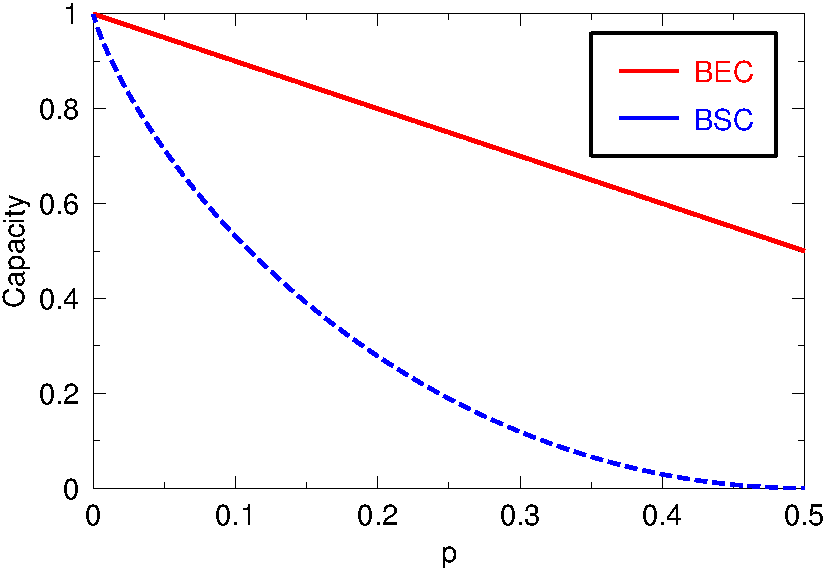
\includegraphics[width=\linewidth]{figures/becbsc.pdf}
\caption{The capacity of the BEC and BSC.}
\label{fig:becbsc}
\end{center}
\end{figure}
In the following we analyze the capacity of a large class of channels. A channel is called weakly symmetric if all rows are permutations of each other and all columns add up to the same value.
\begin{example}
The following transition matrix corresponds to a weakly symmetric channel.
\begin{equation}
\begin{pmatrix}
1/5 & 1/5 & 1/5 & 2/5 &0\\
1/5 & 1/5 & 1/5 & 0 &2/5
\end{pmatrix}
\end{equation}
\end{example}
\begin{lemma}
The capacity of a weakly symmetric channel $N$ is given by:
\begin{equation}
C(N)=\log|Y|-H(\text{row})
\end{equation}
where $|Y|$ is the number of elements of the output alphabet and $H(\text{row})$ is the entropy of one of the rows of the transition matrix.
\end{lemma}
\begin{proof}
\begin{align}
I(X;Y)&=H(Y)-H(Y|X)\\
      &=H(Y)-H(\text{row})\\
      &\leq \log|Y|-H(\text{row})
\end{align}
where the second equality follows because the entropy of $H(Y|x)$ coincides with the entropy of one of the rows of the transition matrix.

Now let us compute the distribution of $Y$ under a uniform distribution on the input. 
\begin{align}
p_Y(y)&=\sum_{x\in X}p_{YX}(y|x)p_X(x)\\
      &=\frac{1}{|X|}\sum_{x\in X}p_{YX}(y|x)\label{eq:sum}
\end{align}
The sum in the right hand side of equation \eqref{eq:sum} corresponds to a column in the transition matrix. In other words, the probability is the same for all $y$ which implies that $Y$ is also uniformly distributed which, in turn, implies that the upper bound on the mutual information can be achieved with a uniform distribution on the input. 
\end{proof}
\booksection{Exercises}
\begin{exercise}
Let $C$ be a linear binary code. Prove that either all codewords have even Hamming weight or half of the codewords have even weight and half odd weight.
\end{exercise}
\begin{exercise}
Find the capacity of a channel given by transition matrix
\begin{equation}
\begin{pmatrix}
1-e&e&0&0\\
  0&0&e&1-e
\end{pmatrix}
\end{equation}
\end{exercise}
\booksection{Solutions to selected exercises}
\begin{solution}[Exercise \ref{ex:bsc}]
\begin{itemize}
\item This is the probability of having no bit flip: $(1-p)^3$.
\item This is the probability of having one of the three bit flipped, there are $3\choose 1$ ways in which this can happen and each one has probability $(1-p)^2p$. Hence: $3(1-p)^2p$.
\item This is the probability of having two of the three bits flipped, there are $3\choose 2$ ways in which this can happen and each one has probability $(1-p)p^2$. Hence: $3(1-p)p^2$.
\item This is the probability of having the three of the three bits flipped, there are $3\choose 3$ ways in which this can happen and it has probability $p^3$. Hence: $p^3$.
\item The decoder will output the wrong guess when there are either two or three errors. Hence the error probability is: $3(1-p)p^2+p^3$.
\end{itemize}
\begin{figure}[h!]
\begin{center}
\def\svgwidth{\columnwidth} 
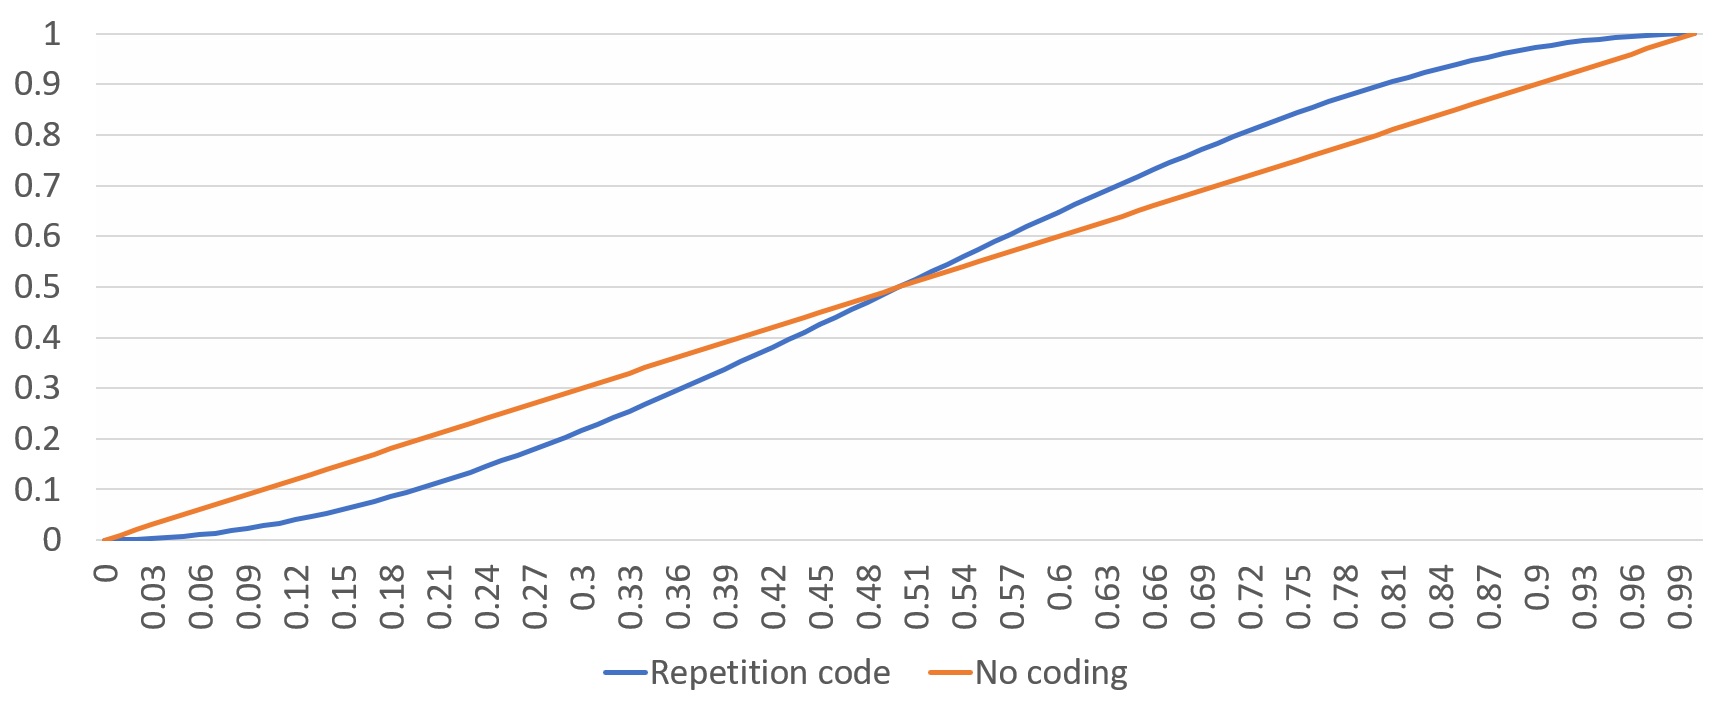
\includegraphics[width=\linewidth]{figures/bscrepcode.png} 
\caption{Decoding error vs crossover probability for the repetition code and for uncoded transmission.}
\label{fig:bscrep}
\end{center}
\end{figure}
\end{solution}
\begin{solution}[Exercise \ref{ex:bec}]
\begin{itemize}
\item This is the probability of having no bit erased: $(1-e)^3$.
\item This is the probability of having one of the three bits erased, there are $3\choose 1$ ways in which this can happen and each one has probability $(1-e)^2e$. Hence: $3(1-e)^2e$.
\item This is the probability of having two of the three bits erased, there are $3\choose 2$ ways in which this can happen and each one has probability $(1-e)e^2$. Hence: $3(1-e)e^2$.
\item This is the probability of having the three of the three bits erased, there are $3\choose 3$ ways in which this can happen and it has probability $e^3$. Hence: $e^3$.
\item Since there are no bit flips, even when there are two erasures, there is a single codeword compatible. When there are three erasures, the decoder has no information but can choose uniformly at random either $(0,0,0)$ or $(1,1,1)$. Hence, the error probability is: $\frac{1}{2}e^3$.
\end{itemize}
\begin{figure}[h!]
\begin{center}
\def\svgwidth{\columnwidth} 
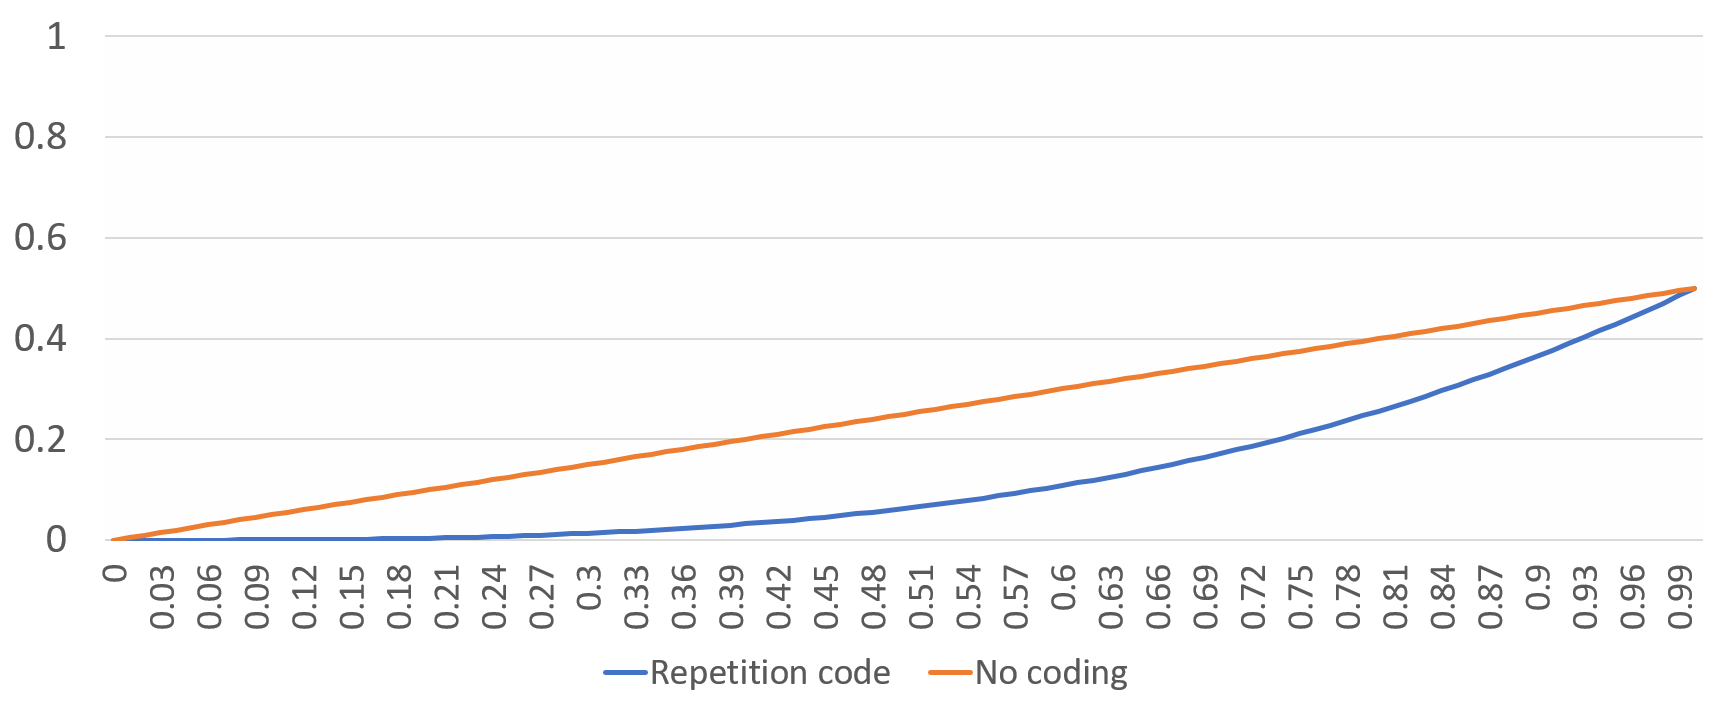
\includegraphics[width=\linewidth]{figures/becrepcode.png} 
\caption{Decoding error vs erasure probability for the repetition code and for uncoded transmission.}
\label{fig:bscrep}
\end{center}
\end{figure}
\end{solution}
\begin{solution}[Exercise~\ref{ex:paritycode}]
\begin{itemize}
\item In order to construct the generator matrix, it is enough to understand the action of the code on a basis of the original space. Let $u_1=(1,0,\ldots,0),u_2=(0,1,0,\ldots,0),\ldots,u_n=(0,\ldots,0,1)$ be the elements of the canonical basis. Since the code maps them to $(1,0,\ldots,0,1),u_2=(0,1,0,\ldots,0,1),\ldots,u_n=(0,\ldots,0,1,1)$, we conclude that the generator matrix is of the form: 
\begin{equation}
G=\begin{pmatrix}
1&0&0&\ldots&0&1\\
0&1&0&\ldots&0&1\\
\vdots &\vdots&\vdots & &\vdots &\vdots\\
0&0&0&\ldots&1&1
\end{pmatrix}=\left(\qquad I_k\qquad\left| \begin{matrix}1\\1\\ \vdots\\ 1\end{matrix}\right.\right)
\end{equation}
\item The minimum distance of this code is two. We can see it by looking at the first $k$ bits of a codeword. If two codewords only differ in one position, that also means that their sum is off by one, hence the last position will also be different. 
\end{itemize}
\end{solution}

\begin{solution}[Exercise~\ref{ex:ycosxcos}]
If $y\in x+C$ then, there exists some codeword $c$ such that $y=x+c$. Moreover, $y+c=x+c+c=x$, hence $x\in y+C$.
\end{solution}
\begin{solution}[Exercise~\ref{ex:cosets}]
Let us first find the coset $0+C$, that is, the set of codewords:
\begin{align}
0+C&=\{\begin{pmatrix}0&0\end{pmatrix}\cdot G,\begin{pmatrix}0&1\end{pmatrix}\cdot G,\begin{pmatrix}1&0\end{pmatrix}\cdot G,\begin{pmatrix}1&1\end{pmatrix}\cdot G\}\\
&=\{\begin{pmatrix}0&0&0&0\end{pmatrix},\begin{pmatrix}0&1&1&1\end{pmatrix},\begin{pmatrix}1&0&0&1\end{pmatrix},\begin{pmatrix}1&1&1&0\end{pmatrix}\}
\end{align}
We can construct the following cosets by adding the set of codewords to low weight vectors:
\begin{align}
\begin{pmatrix}0&0&0&1\end{pmatrix}+C&=\{\begin{pmatrix}0&0&0&1\end{pmatrix},\begin{pmatrix}0&1&1&0\end{pmatrix},\begin{pmatrix}1&0&0&0\end{pmatrix},\begin{pmatrix}1&1&1&1\end{pmatrix}\}\\
\begin{pmatrix}0&0&1&0\end{pmatrix}+C&=\{\begin{pmatrix}0&0&1&0\end{pmatrix},\begin{pmatrix}0&1&0&1\end{pmatrix},\begin{pmatrix}1&0&1&1\end{pmatrix},\begin{pmatrix}1&1&0&0\end{pmatrix}\}\\
\begin{pmatrix}0&1&0&0\end{pmatrix}+C&=\{\begin{pmatrix}0&1&0&0\end{pmatrix},\begin{pmatrix}0&0&1&1\end{pmatrix},\begin{pmatrix}1&1&0&1\end{pmatrix},\begin{pmatrix}1&0&1&0\end{pmatrix}\}
\end{align}
\end{solution}
\begin{solution}[Exercise~\ref{ex:sadec1}]
If $y$ and $t$ belong to the same coset this means that they there exists some $x\in\{0,1\}^n$ and $c_1,c_2\in C$ such that $y=x+c_1$ and $t=x+c_2$. Then $t+y=x+c_1+x+c_2=c_1+c_2$, moreover since $C$ is a vector space $c_1+c_2\in C$. That is, $t+y$ is a codeword. 
\end{solution}
\begin{solution}[Exercise~\ref{ex:sadec2}]
Recall that upon receiving $y$, the standard array decoder output $y+t$ where $t$ is a coset leader of $y+C$.

Suppose that there exists a codeword $c'$ such that $d(y,c')<d(y,y+t)$. We can rewrite it as $w(t')<w(t)$ where $t'=y+c'$. However, note that $t'\in y+C$, which is a contradiction since $t'$ can not have smaller weight than a coset leader. 

Note that there is a small subtlety in the sense that when more than one codeword is at minimum distance, the standard array based decoder will not choose the codeword uniformly at random.
\end{solution}
\begin{solution}[Exercise~\ref{ex:cbsc}]

In the binary symmetric channel the two symbols of the input alphabet are either perfectly transmitted with probability $1-p$ or flipped with probability $p$. 

Consider an arbitrary distribution on the input symbols and the associated random variable $X$. Let us first find the mutual information between the input $X$ and the induced random variable at the output of the channel $Y$~\cite{Cover_91}:

\begin{align}
I(X;Y) &= H(Y) - H(Y|X) \\
       &= H(Y) - \sum_x p(x)H(Y|x) \\
       &= H(Y) - \sum_x p(x)H(p,1-p) \\
       &= H(Y) - H(p,1-p)\sum_x p(x) \\
       &\leq 1 - H(p,1-p)\label{eq:bscC} 
\end{align}
where the upper bound follows from $Y$ being a binary random variable.

If we can find a distribution on the input symbols that achieve the upper bound we show that the upper bound is the capacity of the channel. Consider a uniform distribution on the input and let us find the induced distribution at the output of the channel:
\begin{align}
p_Y(0)&=p_{YX}(0,0)+p_{YX}(0,1)\\
      &=p_{X}(0)p_{YX}(0|0)+p_{X}(1)p_{YX}(0|1)\\
      &=\frac{1}{2}(1-p)+\frac{1}{2}p\\
      &=\frac{1}{2}
\end{align}
and $p_Y(1)=1-p_Y(0)=\frac{1}{2}$. In consequence, if the input symbols are uniformly distributed $H(Y)=1$ and the upper bound is achieved.
\end{solution}
\begin{solution}[Exercise~\ref{ex:cbec}]

Consider an arbitrary distribution on the input $p_X(0)=x,p_X(1)=1-x$. Let us find what is the induced probability at the output. 
\begin{align}
p_Y(0)&=p_{YX}(0,0)+p_{YX}(0,1)\\
      &=p_{X}(0)p_{YX}(0|0)+p_{X}(1)p_{YX}(0|1)\\
      &=x(1-p)\ ,
\end{align}
\begin{align}
p_Y(1)&=p_{YX}(1,0)+p_{YX}(1,1)\\
      &=p_{X}(0)p_{YX}(1|0)+p_{X}(1)p_{YX}(1|1)\\
      &=(1-x)(1-p)
\end{align}
and
\begin{align}
p_Y(e)&=p_{YX}(e,0)+p_{YX}(e,1)\\
      &=p_{X}(0)p_{YX}(e|0)+p_{X}(1)p_{YX}(e|1)\\
      &=xp+(1-x)p\\
      &=p\ .
\end{align}

Now we will find $H(X|Y)$. For this we need the conditional distributions on the input alphabet for each value of the output alphabet.  
\begin{align}
p_{XY}(0|0)&=\frac{p_{XY}(00)}{p_Y(0)}\\
           &=\frac{p_{YX}(0|0)p_X(0)}{p_Y(0)}\\
           &=\frac{(1-p)x}{(1-p)x}\\
           &= 1, 
\end{align}
which implies $P_{XY}(1|0)=0$. Similarly, $P_{XY}(1|1)=1$ and $P_{XY}(0|1)=0$. Finally, for $e$:
\begin{align}
p_{XY}(0|e)&=\frac{p_{XY}(0e)}{p_Y(e)}\\
           &=\frac{p_{YX}(e|0)p_X(0)}{p_Y(e)}\\
           &=\frac{px}{p}\\
           &= x 
\end{align}
and $p_{XY}(1|e)=1-x$.

We can now develop $H(X|Y)$:
\begin{align}
\label{eq:beccap}
H(X|Y) &= x(1-p )H(X|Y=0) \nonumber\\
           & + p H(X|Y=e)\nonumber\\
           & + (1-x)(1-p)H(X|Y=1) \\
           &=pH(x,1-x)
\end{align}
\noindent The second equality holds from $H(X|Y=1)=H(X|Y=0)=0$. We can now plug Eq.~\ref{eq:beccap} in Eq.~\ref{eq:mutualinformation} and bound from above the mutual information:
\begin{align}
I(X;Y) &= H(X) - H(X|Y) \\
         &= H(x, 1-x) - pH(x, 1-x)\\
         & \leq  1 - p\label{eq:becineq}
\end{align}
\noindent equality in Eq.~\ref{eq:becineq} is achieved again by the uniform distribution. That is, for $x=\frac{1}{2}$.
\end{solution}
\booksection{Further reading}
We have covered in this chapter several topics on data transmission. For a quick introduction to coding theory, we refer to the first chapter in MacKay \cite{mackay2003information} and to section 7.11 in Cover and Thomas \cite{Cover_91}. For a more in depth introduction to coding theory, we refer to the book by Hill \cite{hill1986first}.

For the noisy channel theorem and computing capacity we refer to chapters 9 and 10 in MacKay \cite{mackay2003information} and to chapter 7 in Cover and Thomas \cite{Cover_91}. 

Finally, the treatment of the noisy channel theorem in this class, does not follow the common structure via typical sequences but instead it is based on the extremely concise proof in \cite{lomnitz2012simpler}.

\iffalse
\booksection{Sketch of the noisy channel theorem}

The capacity of a channel specifies the maximum rate at which a source can be reliably sent through a channel. On the other hand, no source with a rate over the capacity of the channel can be sent with a vanishing error probability.

\begin{figure}
\begin{center}
\def\svgwidth{\columnwidth} 
\input{figures/channel.pdf_tex} 
\caption[Jointly typical sequences]{Graphical representation of the input and output typical sequences. A good encoding chooses as codewords a subset of the input typical sequences that produces disjoint sets of output typical sequences.}
\label{fig:channel}
\end{center}
\end{figure}

A sketch of the proof would be as follows. Encoder and decoder share a code-book of $2^{nR}$ codewords chosen within the $2^{nH(X)}$ typical sequences~\cite{Massey_77}. The encoder sends a codeword ${x}$ drawn with uniform probability. The decoder outputs a word $\hat{{x}}$ jointly typical with the received word ${y}$. It declares an error if ${x}$, ${y}$ are not jointly typical and a decoding error can occur if there exists ${x}'\neq {x}$ jointly typical with ${y}$. We know by Eq.~\ref{eq:jointtypical} that the probability of non-joint typicality for long enough $n$ can be made as small as desired. %We can bound the second source of error $p_e$ as well:

%\begin{eqnarray}
%p_e &\leq&  \left( 2^{nR}-1 \right) \frac{2^{n(H({XY})-\delta )}}{2^{n(H(X)-\delta )}2^{n(H(Y)-\delta )}}\nonumber\\
%     &\leq & 2^{-n(I(X;Y)-R-3\delta)}
%\end{eqnarray}
%\noindent in the first inequality we have bounded the error probability as the probability that one among the $2^{nR-1}$ remaining codewords belongs to the set of jointly typical sequences. The error probability vanishes only if $R<I(X;Y)$. However, we did not impose any condition on the $p(x)$ in the above discussion. In other words, if we choose the distribution that maximizes $I(X;Y)$, the typical sequence encoding achieves the capacity of the channel.

The intuition behind the achievability proof is simple. The decoder has access to two sets: the set of sequences jointly typical with ${y}$, and the set of codewords. If the intersection is to be a single word, every codeword has to be jointly typical with a disjoint set of typical output words. 

Approximately, every codeword is jointly typical with $2^{nH(Y|X)}$ words. Then the number of jointly typical output words with input codewords is upper bounded by $2^{nR+nH(Y|X)}$, where $R$ is the coding rate. This number should be much smaller than the total number of typical sequences $2^{nH(Y)}$:
 
\begin{equation*}
2^{nR+nH(Y|X)} < 2^{nH(Y)}
\end{equation*}

\noindent which operating returns the expected result:

\begin{equation*}
R < I(X;Y)
\end{equation*}

In conclusion, as long as the coding rate is below the mutual information between input and output for $n$ long enough we can construct a code that allows the decoder to distinguish between codewords with a vanishing probability of error.
\fi

